\chapter{Формат ключевого контейнера}\label{CONT}

\section{Правила защиты}\label{CONT.Rules}

Контейнер программного КТ содержит личный ключ СТБ~34.101.45.
Контейнер может защищаться на пароле~--- строке в естественном алфавите. 
Строку должен суметь запомнить владелец личного ключа, и поэтому пароль 
обычно имеет сравнительно небольшую длину, низкую энтропию, его 
определение путем перебора намного проще, чем определение личного ключа с 
помощью известных криптоаналитических атак. 

Чтобы сохранить стойкость личного ключа при хранении, контейнер должен
дополнительно защищаться аппаратно. Например, контейнер может храниться
внутри устройства, доступ к объектам которого осуществляется только после 
предъявления пароля, причем доступ блокируется после нескольких неверных 
попыток ввода пароля. Для сравнения, блокировать ввод пароля при прямом 
доступе к контейнеру нельзя.  

Если дополнительная защита контейнера затруднена, то вместо 
низкоэнтропийного пароля следует использовать высокоэнтропийный ключ~--- 
случайное двоичное слово~$P$ длины~$l\in\{128,192,256\}$, где~$l$~--- 
уровень стойкости личного ключа.  
%
Ключ защиты следует разделить на несколько частичных секретов с помощью 
алгоритма, определенного в СТБ 34.101.60 (п. 7.3). 

Частичые секреты также являются двоичными словами длины~$l$. Их количество не 
должно превышать~$16$. Пороговое число (минимальное число частичных секретов,
необходимых для восстановления ключа) должно быть не меньше~$2$.
%
При разделении должны использоваться стандартные открытые 
ключи, заданные в СТБ 34.101.60 (приложение A). При этом с каждым 
частичным секретом связывается определенный открытый ключ одной из 
таблиц~A.2, A.3, A.4 приложения.  
%
Номер открытого ключа считается номером частичного секрета.
Номер кодирует октетом: октет $\hex{01}$ представляет номер~$1$, 
октет~$\hex{02}$~--- номер~$2$,\ldots, октет~$\hex{10}$~--- номер~$16$.
Октет номера записывается в начало частичного секрета и хранится вместе с 
ним.

Частичные секреты размещаются на различных носителях информации 
владельца, в нескольких его сетевых репозиториях. 
%
Размещение должно быть организовано так, чтобы несанкционированный 
доступ к пороговому числу частичных секретов был максимально затруднен.

Частичные секреты могут сохраняться во вспомогательных контейнерах, 
защищенных на паролях. Пароли защиты различных контейнеров могут совпадать.
В любой комбинации порогового числа частичных секретов хотя бы один из них 
должен быть защищен на пароле.

Ключ~$P$ защиты контейнера с личным ключом кодируется текстовой
строкой~$\texttt{hex}(P)$ длины~$l/4$.
%
Таким образом, для защиты контейнера любого типа всегда используется 
секретная строка: либо пароль, либо закодированный ключ.

Частичный секрет, который хранится в открытом виде, также может 
кодироваться текстовой строкой. Эта строка будет иметь длину~$l/4+2$.
Первые два символа строки представляют номер секрета.

Формат ключевого контейнера описывается 
типом~\texttt{EncryptedPrivateKeyInfo}, определенным в~\ref{CONT.CT}.
Контейнер~\texttt{EncryptedPrivateKeyInfo} содержит защищенный вложенный
контейнер, в котором непосредственно хранится личный ключ или частичный 
секрет (см. рисунок~\ref{Fig.CONT.1}). Формат вложенного контейнера 
описывается типом~\texttt{PrivateKeyInfo}, определенным в~\ref{CONT.PT}.

\begin{figure}[hbt]
\begin{center}
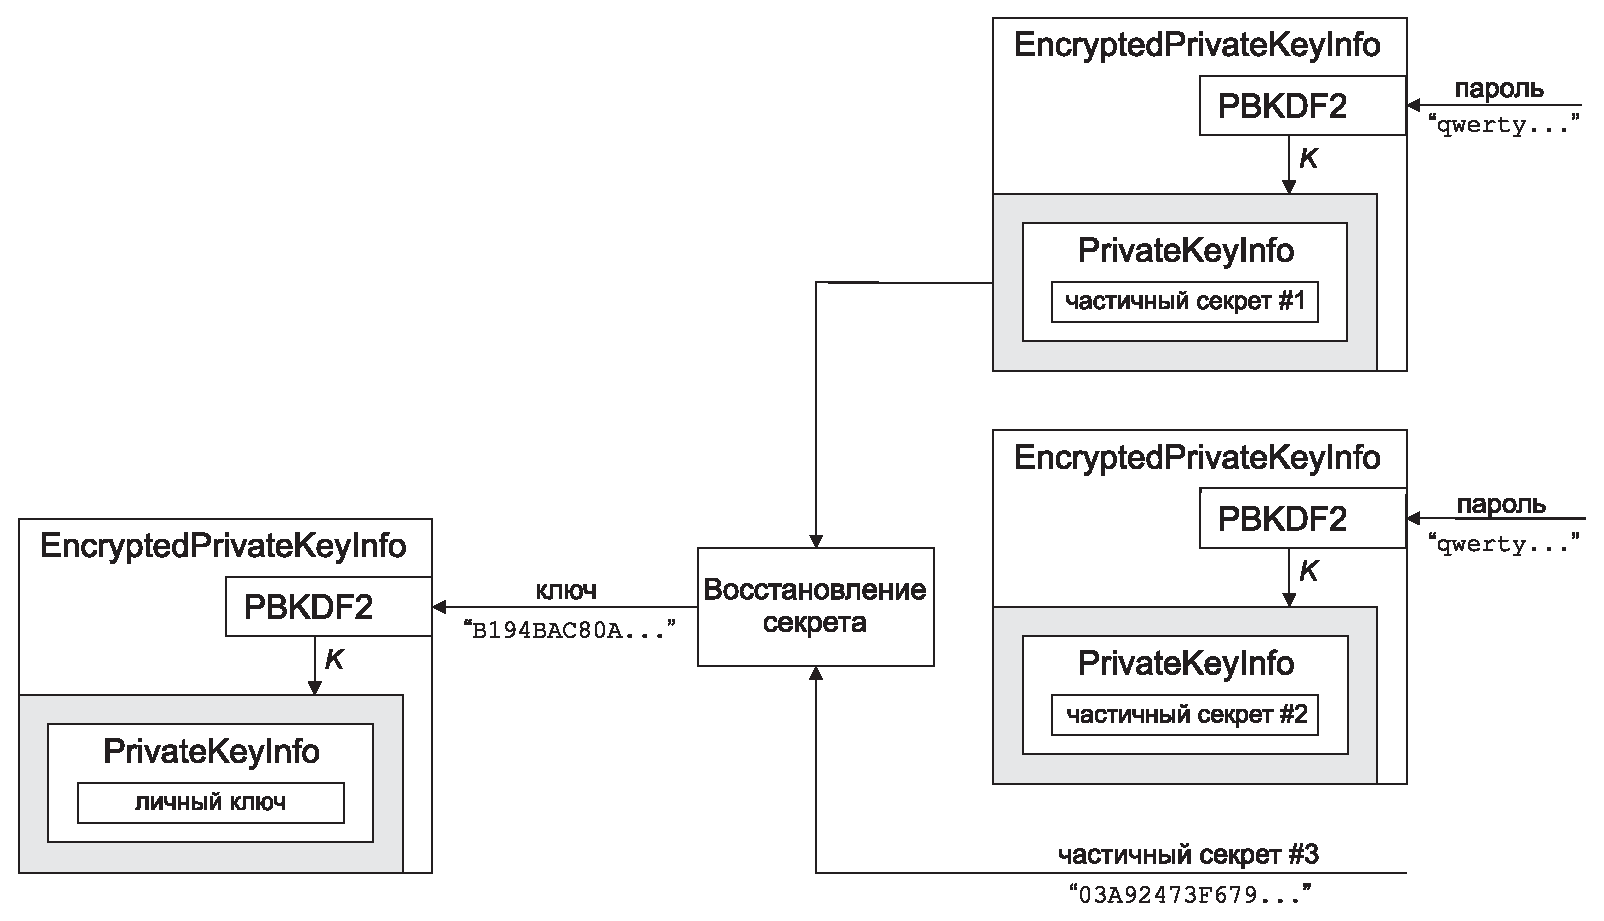
\includegraphics[width=15cm]{../figs/cont}
\end{center}
\caption{Защита ключевого контейнера}
\label{Fig.CONT.1}
\end{figure}

\section{Установка защиты}\label{CONT.Wrap}

Контейнер~\texttt{PrivateKeyInfo} защищается на секретной строке и
встраивается в контейнер~\texttt{EncryptedPrivateKeyInfo} следующим
образом.
\begin{enumerate}
\item
Входная секретная строка кодируется строкой октетов по правилам 
UTF-8~\cite{UTF8}. 
\item
По полученной строке строится ключ~$K\in\{0,1\}^{256}$.
Для этого используется алгоритм PBKDF2, определенный в~\cite{PKCS5} и 
конкретизированный в СТБ 34.101.45 (п.~E.2).
\item
Контейнер \texttt{PrivateKeyInfo} кодируется по базовым правилам (BER).
В результате кодирования получается строка октетов~$X\in\{0,1\}^{8*}$.
\item
Cтрока~$X$ защищается с помощью алгоритма \texttt{belt-keywrap}, 
определенного в СТБ 34.101.31 (п.~6.8.3). 
На вход алгоритма подаются~$X$, нулевой заголовок~$I\in\{0,1\}^{128}$
и~ключ~$K$, построенный на шаге~2. Алгоритм возвращает защищенную 
строку~$Y\in\{0,1\}^{|X|+128}$. 
\item
Строка~$Y$ записывается в компонент~\texttt{encryptedData}
контейнера~\texttt{EncryptedPrivateKeyInfo} (см.~\ref{CONT.CT}).
Остальные компоненты контейнера
заполняются служебной информацией и параметрами~PBKDF2.
\end{enumerate}

\section{Снятие защиты}\label{CONT.Unwrap}

Снятие защиты с контейнера~\texttt{EncryptedPrivateKeyInfo} 
означает определение вложенного контейнера~\texttt{PrivateKeyInfo} 
в открытом виде. Защита снимается на той же секретной строке, которая 
использовалась при установке защиты. 
Снятие защиты выполняется следующим образом.
\begin{enumerate}
\item
Входная секретная строка кодируется строкой октетов по правилам  
UTF-8~\cite{UTF8}. 
\item
По полученной строке с помощью алгоритма PBKDF2
вычисляется ключ~$K\in\{0,1\}^{256}$.
Параметры PBKDF2 предварительно считываются из контейнера.
\item
Определяется строка октетов~$Y\in\{0,1\}^{8*}$, размещенная в 
компоненте~\texttt{encryptedData} контейнера. 
\item
Строка~$Y$ обрабатывается алгоритмом~$\texttt{belt-keywrap}^{-1}$, определенным 
в СТБ 34.101.31 (п.~6.8.4). На вход алгоритма подаются~$Y$, 
нулевой заголовок~$I\in\{0,1\}^{128}$ и ключ~$K$, построенный на шаге~$2$.
Алгоритм возвращает открытую строку~$X\in\{0,1\}^{|Y|-128}$ или 
признак~\texttt{ОШИБКА}. Возврат признака~\texttt{ОШИБКА} означает, что 
либо нарушена целостность контейнера, либо входная секретная строка неверна.  
При возврате признака снятие защиты преждевременно завершается с ошибкой.
\item
Строка~$X$ интерпретируется как BER-код 
контейнера~\texttt{PrivateKeyInfo}. Строка декодируется, определяется 
вложенный контейнер. 
\end{enumerate}

Снятие защиты завершается с ошибкой не только на шаге 4, но и на 
шагах 2, 3, 5 при несоблюдении форматов~\texttt{EncryptedPrivateKeyInfo} 
и~\texttt{PrivateKeyInfo}. 

\section{Тип \texttt{PrivateKeyInfo}}\label{CONT.PT}

Тип~\texttt{PrivateKeyInfo} определен в~\cite{PKCS8}.
В настоящем стандарте он конкретизируется следующим образом.

\begin{verbatim}
PrivateKeyInfo ::= SEQUENCE {
  version                  INTEGER(0),
  keyAlgorithm             CHOICE {
    bignPrivkeyAlgorithm   BignAlgorithmIdentifier,
    belsSharekeyAlgorithm  BelsAlgorithmIdentifier },
  key                      OCTET STRING }

BignAlgorithmIdentifier ::= SEQUENCE {
  algorithm  OBJECT IDENTIFIER(bign-pubkey),
  params     OBJECT IDENTIFIER(bign-curve256v1 | bign-curve384v1 | 
                               bign-curve512v1) }

BelsAlgorithmIdentifier ::= SEQUENCE {
  algorithm  OBJECT IDENTIFIER(bels-share),
  params     OBJECT IDENTIFIER(bels-m0128v1 | bels-m0192v1 | bels-m0256v1) }
\end{verbatim}

Компонент~\texttt{keyAlgorithm} выбирается двумя способами:
выбор~\texttt{bignPrivkeyAlgorithm} означает, что в контейнере хранится личный 
ключ, выбор~\texttt{belsSharekeyAlgorithm}~--- частичный секрет. 

Компонент \texttt{bignAlgorithm} идентифицирует личный ключ и параметры 
эллиптической кривой, к которым он привязан. Могут использоваться
только стандартные параметры, определенные в СТБ 34.101.45 (приложение Б). 
%
Задействованные идентификаторы~\texttt{bign-pubkey}, 
\texttt{bign-curve256v1}, \texttt{bign-curve384v1} 
и~\texttt{bign-curve512v1} определены в СТБ~34.101.45 (приложение Д).

Аналогичным образом компонент~\texttt{belsAlgorithm} идентифицирует 
частичный секрет и долговременный общий открытый ключ. 
Могут использоваться только стандартные общие ключи, 
определенные в СТБ 34.101.60 (приложение А). 
Идентификаторы \texttt{bels-share}, \texttt{bels-m0128v1}, 
\texttt{bels-m0192v1}, \texttt{bels-m0256v1} определены в СТБ 34.101.60 
(приложение Г).

Личный ключ или частичный секрет хранятся в компоненте \texttt{key}
в виде строки октетов. Длина строки должна соответствовать уровню
стойкости~$l$, который определяется по стандартным параметрам
(эллиптической кривой или общему открытому ключу).

Строка личного ключа строится по правилам СТБ 34.101.45 (п. 5.4). 
Строка состоит из $l/4$ октетов. 
%
Строка частичного секрета состоит из~$l/8+1$ октетов. 
Первый октет представляет номер частичного секрета (см.~\ref{CONT.Rules}).

\section{Тип \texttt{EncryptedPrivateKeyInfo}}\label{CONT.CT}

Тип~\texttt{EncryptedPrivateKeyInfo} определен в~\cite{PKCS5}. В настоящем
стандарте он конкретизируется следующим образом.

\begin{verbatim}
EncryptedPrivateKeyInfo ::= SEQUENCE {
  encryptionAlgorithm  EncryptionAlgorithmIdentifier,
  encryptedData        OCTET STRING }

EncryptionAlgorithmIdentifier ::= SEQUENCE {
  algorithm   OBJECT IDENTIFIER(id-PBES2),
  params      PBES2-params }

PBES2-params ::= SEQUENCE {
  keyDerivationFunc PBKDF2AlgorithmIdentifier,
  encryptionScheme  BeltKeywrapAlgorithmIdentifier }

PBKDF2AlgorithmIdentifier ::= SEQUENCE {
  algorithm   OBJECT IDENTIFIER(id-PBKDF2),
  params      PBKDF2-params }

BeltKeywrapAlgorithmIdentifier ::= SEQUENCE {
  algorithm   OBJECT IDENTIFIER(belt-keywrap256),
  params      NULL }

PBKDF2-params ::= SEQUENCE {
  salt            OCTET STRING(SIZE(8)),
  iterationCount  INTEGER (10000..MAX),
  prf             PrfAlgorithmIdentifier }

PrfAlgorithmIdentifier ::= SEQUENCE {
  algorithm OBJECT IDENTIFIER(hmac-hbelt), 
  params    NULL }

\end{verbatim}

Компонент~\texttt{encryptedData} типа \texttt{EncryptedPrivateKeyInfo}
представляет защищенный вложенный контейнер, 
а компонент~\texttt{encryptionAlgorithm} описывает
алгоритмы защиты и их параметры. 

Задействованные в описаниях идентификаторы~\texttt{id-PBES2} 
и~\texttt{id-PBKDF2} определены в~\cite{PKCS5}, а также в СТБ~34.101.45 
(приложение Е).  
%
Идентификатор~\texttt{belt-keywrap256} алгоритмов 
$\texttt{belt-keywrap}$, $\texttt{belt-keywrap}^{-1}$
с $256$-битовыми ключами определен в СТБ 34.101.31 (приложение Б).

Тип~\texttt{PBKDF2-params} описывает параметры PBKDF2.
Введенные в описание ограничения соответствуют 
рекомендациям СТБ~34.101.45 (п. E.4).
%
В частности, для имитозащиты должен использоваться алгоритм HMAC, 
определенный в~СТБ~34.101.47 (п. 6.1), c функцией хэширования, 
определенной в СТБ 34.101.31 (п. 6.9). 
Идентификатор~\texttt{hmac-hbelt} этого алгоритма 
определен в СТБ 34.101.47 (приложение~Б).

